\documentclass[11pt]{article}

\usepackage{hyperref}
\usepackage{geometry}
\usepackage[T1]{fontenc}
\usepackage{natbib}
\usepackage{changepage}

% Misc packages
\usepackage{graphicx}
\usepackage{amsmath, amssymb}

% Units
\newcommand{\msun}{\textrm{M}_\odot}
\newcommand{\kpc}{\textrm{kpc}}
\newcommand{\kms}{\ensuremath{\textrm{km}~\textrm{s}^{-1}}}
\newcommand{\masyr}{\ensuremath{\textrm{mas}~\textrm{yr}^{-1}}}

% Astronomy
\newcommand{\feh}{\ensuremath{[\textrm{Fe} / \textrm{H}]}}

% page size
\geometry{
  body={6.5in, 9in},
  left=1.0in,
  top=1.0in,
  nohead,
  nofoot
}

% Title stuff
\let\apwtitle\title
\renewcommand{\apwtitle}[1]{\title{
	\vspace{-6ex}
        {\fontsize{12pt}{0em}\selectfont \textbf{#1}}
        \vspace{-6.5ex}
}}

% Change section font size and spacing
\usepackage[small,compact]{titlesec}
\titleformat{\section}{\normalfont\fontsize{12pt}{0em}\bfseries}{\thesection}{12pt}{}
\titleformat{\subsection}{\normalfont\fontsize{12pt}{0em}\bfseries}{\thesubsection}{0.5em}{}
\titleformat{\subsubsection}{\normalfont\fontsize{12pt}{2em}\bfseries}{}{0.em}{}
\titlespacing{\section}{0em}{8pt}{2pt}
\titlespacing{\subsection}{0.em}{4pt}{2pt}
\titlespacing{\subsubsection}{0em}{2pt}{2pt}

\pagenumbering{gobble}
% \setlength{\parskip}{\baselineskip}%
\setlength{\parskip}{6pt}
\setlength{\parindent}{0pt}%

\apwtitle{Deep imaging of the GD-1 stellar stream with HSC -- A. Price-Whelan et al.}
\date{}
\author{}

\setlength{\bibsep}{0pt plus 0.3ex}

\begin{document}
\maketitle

\vspace{-1em}
The clustering of dark matter (DM) on scales smaller than dwarf galaxies remains one of the most pressing unknowns in cosmology and galaxy formation (Bullock \& Boylan-Kolchin 2017).
Different DM theories predict different minimum mass scales for clustering: In the $\Lambda$CDM model, DM subhalos with negligible baryonic content are expected to exist with arbitrarily low masses, while alternative models (e.g., WDM, SIDM) have larger cut-off masses in the DM power spectrum that depend on the parameters of these models (e.g., Bode et al. 2001): The mere existence of low-mass substructure therefore constrains the physics of dark matter. % (Springel et al. 2008)

Within the stellar halo of our Galaxy, stellar streams---e.g., remnants of disrupted globular clusters (Grillmair \& Carlin 2016)---are a unique and powerful way to test small-scale predictions from DM theories:
A gravitational encounter between a stream and a massive perturber (e.g., a DM subhalo) produces density variations along the stream and can create morphological features such as gaps, spurs, and loops of debris (Yoon et al. 2011). %that are not expected in models for stream formation in a smooth halo.
We recently showed that the GD-1 stellar stream has at least 2 gaps and a ``spur'' of debris emanating from one gap (Price-Whelan \& Bonaca 2018), which can plausibly be explained by a perturbation from a massive substructure (Bonaca et al. 2019).
Deeper imaging is now needed to measure the density contrast of these gaps and to confirm the existence of the spur, both of which will enable constraints on the mass and size of the perturber.

% \section*{The GD-1 stream: a perturbed stream in the Milky Way halo}
\textbf{GD-1 perturbations as possible tracers of small-scale dark matter physics:}
The GD-1 stellar stream, which spans heliocentric distances $d\sim 8$--$12~\textrm{kpc}$, was discovered using photometry from the Sloan Digital Sky Survey (Grillmair \& Dionatos 2006) and has a stellar population (age $\sim 12~\textrm{Gyr}$) and width consistent with being a fully-disrupted globular cluster (Koposov et al. 2010).
% GD-1 has been used to measure the mass and shape of the large-scale mass distribution within the Galaxy (Koposov et al. 2010; Bovy et al. 2016).
% Recently, using CFHT/Megacam imaging over a $\sim 45^\circ \times 0.8^\circ$ footprint centered on the stream, de Boer at al. (2018) detected density variations along the stream and possible deviations of the main stream track that are not expected from simple models of the stream formation.
% Recently, de Boer et al. (2018) detected tentative density variations along the stream using CFHT/Megacam imaging
% However, despite reaching depths of $g \sim 24$, the study only used sources brighter than $g \sim 23$ because of star--galaxy confusion.
Using astrometry from the \textit{Gaia} mission (DR2) and photometry from Pan-STARRS, we recently mapped GD-1 over $\sim 100^\circ$ on the sky (Figure~1, bottom panel), producing the highest-contrast view of a thin stellar stream to date (Price-Whelan \& Bonaca 2018).
% Figure~1 (lower panel) shows a $60^\circ$ segment of the stream selected with \textit{Gaia} + PS1: black markers show the sky positions (in GD-1 coordinates) of individual stars identified as probable stream members, with some background contamination throughout the field.
This new view of the stream reveals at least two significant under-densities or ``gaps'' along the stream (Figure~1, lower), one of which has an associated spur of stars that lies parallel to, but offset by $\sim1^\circ$ from, the main stream (Gap 1 and over-density labeled ``Spur''; Figure 1).

% Gaps in stellar streams with large density drops can only be formed through gravitational encounters (which can leave multiple gaps), or through the final disruption of the progenitor system (which can only explain one gap).
Gaps and spurs in stellar streams can be formed through gravitational encounters:
\emph{The existence of two or more large gaps in GD-1 and the presence of stream stars off of the main stream track strongly suggest that GD-1 has encountered at least one massive perturber.}
GD-1 is the first and only stream for which evidence of strong interactions with substructure have been identified, yet none of the known satellites of the Milky Way have orbits that recently cross near GD-1 (Bonaca et al. 2019):
The GD-1 stream is therefore a promising probe of small-scale dark matter physics.

To constrain the perturber properties requires kinematic measurements of and a confirmation of the existence of the spur, as well as measurements of the density profiles of the gaps (subhalo gaps have characteristic ``horn''-shaped density profiles; Figure~1, upper right panel).
In a separate program, we are obtaining spectroscopy for stars in the GD-1 spur to compliment \textit{Gaia} astrometry (Hectochelle/MMT; PI Bonaca).
% These density profiles encode properties of the perturber (mass and density), the geometry of the encounter (angle, impact parameter, and relative velocity), and the time of the encounter (e.g., Erkal \& Belokurov 2015).
% However, the stellar mass in these features and the density variations along streams are typically small relative to the background stellar density in our Galaxy: for a perturber mass $M \gtrsim 10^7~\msun$, and an encounter within the last orbital period, the density contrast between the horns and the stream is typically $\rho/\rho_0 \gtrsim 1.2$.
To measure the density profiles of the gaps and to confirm the existence of the spur requires deeper photometry to obtain higher signal-to-noise stellar density measurements.
Gap density variations are typically small relative to the background: For a perturber mass $M \gtrsim 10^7~\msun$, and an encounter within the last orbital period, the density contrast between the horns and the stream is typically $\Delta\rho/\rho_0 \gtrsim 0.2$, but this density contrast is very sensitive to the perturber mass (Figure~1, upper right panel).
\emph{Characterizing the detailed density structure of GD-1 therefore requires deep but wide-area photometric observations.}

\textbf{HSC will enable high signal-to-noise measurements of GD-1 gap profiles:}
We propose to obtain deep $g$- and $i$-band imaging in 17 HSC fields along the GD-1 stream and spur (Figure~1, red circles) to measure density variations along the stream.
These fields are designed to cover the stream, spur, and two gaps, while covering known, dense parts of the stream to use as tests for our member selection (matched-filtering) and density modeling.
We estimate the expected background contamination (stars and galaxies) in each proposed field using point sources from a single HSC-SSP field at a comparable Galactic latitude to GD-1. % (\texttt{i\_extendedness\_value == 0})
To estimate the signal-to-noise (S/N) of the stream, we use a 12 Gyr, $[\textrm{Fe}/\textrm{H}] = -1.4$ luminosity function normalized to the number of \textit{Gaia}+PS1 selected stream stars in a $1.5^\circ \times 1.5^\circ$ field centered at $(\phi_1, \phi_2) = (-35, 0)^\circ$.
Figure~1 (top left) shows a simulated color-magnitude diagram (CMD) for this HSC field assuming a limiting $g$-band magnitude of $g \sim 25.5$.
Figure~1 (top middle) shows the S/N of the stream in an HSC field from matched-filtering in the $g-i$ vs. $g$ CMD for 3 survey limiting magnitudes: PS1 $g \sim 22.5$, Megacam $g \sim 24$, and the proposed HSC observations $g \sim 25.5$.
To measure, e.g., a 20\% density contrast, we need to reach a density $\textrm{S}/\textrm{N} = 30$ per field, which depends on SSP-like seeing to perform high-efficiency star-galaxy separation.
\emph{HSC is the only instrument with sufficient area and sensitivity to efficiently survey multiple gaps in the GD-1 stream and provide a high enough signal-to-noise to measure gap density profile variations expected from an encounter with a low-mass dark matter subhalo.}
The proposed data will (1) definitively rule whether either of the gaps in GD-1 are a consequence of a gravitational encounter, and, if so, (2) combined with a kinematic profile of the gap (from an ongoing Hectochelle/MMT program), will constrain the mass of the perturber to $\sim 20\%$--$40\%$ (e.g., Table~2, Erkal \& Belokurov 2015b).
% We propose to observe 13 HSC fields along the GD-1 stream, covering two significant gaps (Figure~1, bottom panel, red circles).

\begin{figure}[t]
\begin{center}
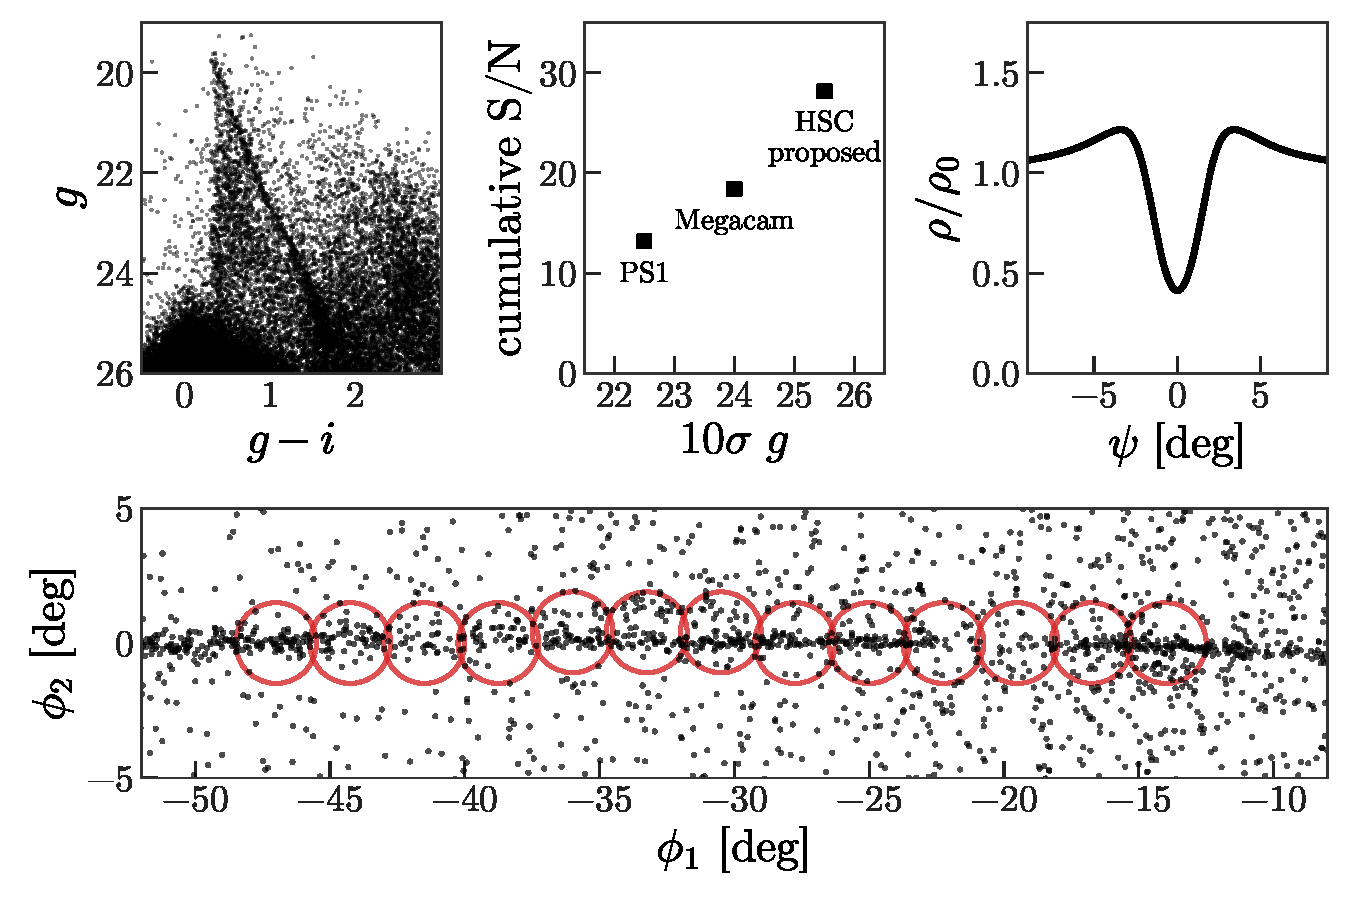
\includegraphics[width=0.75\textwidth]{figure1.pdf}
\caption{
\textbf{Top left:} Simulated GD-1 stellar population in one HSC field super-imposed over point sources from one HSC-SSP field.
\textbf{Top middle:} Expected cumulative signal-to-noise in measuring the spatial density of the stream in one HSC field vs. limiting $g$ magnitude for different surveys.
\textbf{Top right:} Predicted gap density profiles for subhalo encounters with a GD-1 like stream.
\textbf{Bottom:} GD-1 candidate member stars (black markers) with proposed HSC pointings indicated (red circles).
}
\vspace{-2.2em}
\label{fig:}
\end{center}
\end{figure}

{\footnotesize
\textbf{References:}
Bode et al. 2001, ApJ, 556, 93 ---
% Bonaca \& Hogg 2018, arXiv:1804.06854 ---
Bullock \& Boylan-Kolchin 2017, ARAA, 55, 343 ---
% de Boer et al. 2018, MNRAS, 477, 1893 ---
Bonaca et al. 2019, arxiv:1811.03631 ---
Erkal \& Belokurov 2015a, MNRAS, 450, 1136 ---
Erkal \& Belokurov 2015b, MNRAS, 454, 3542 ---
Grillmair \& Dionatos 2006, ApJ, 643, L17 ---
Grillmair \& Carlin 2016, arXiv:1603.08936 ---
Koposov et al. 2010, ApJ, 712, 260 ---
Price-Whelan \& Bonaca 2018, ApJL, 863, L20 ---
% Springel et al. 2008, MNRAS, 391, 1685 ---
Yoon et al. 2011, ApJ, 731, 58}


\end{document}
